\documentclass[a4paper]{article}
\usepackage[14pt]{extsizes} 
\usepackage[T2A]{fontenc}
\usepackage[utf8]{inputenc}
\usepackage{natbib}
\usepackage{graphicx}
\usepackage{amsmath}
\usepackage[english, russian]{babel}
\usepackage{amsmath,amsfonts,amssymb,amsthm,mathtools,mathrsfs}
\usepackage{icomma}
\usepackage{fullpage}
\usepackage{ulem}
\usepackage{eufrak}
\usepackage{setspace}
\usepackage{listings}
\usepackage{indentfirst}
\usepackage[left=2cm,right=1.5cm,top=2cm,bottom=2cm]{geometry}
\usepackage{xcolor}
\usepackage{float}
\usepackage{csquotes}

\setlength{\parindent}{5ex}
\setlength{\parskip}{1em}
\renewcommand{\baselinestretch}{1}

\graphicspath{{images/}}

\definecolor{buzzlightyear}{HTML}{8757A5}
\definecolor{grass}{HTML}{738D06}
\definecolor{literal}{HTML}{F18A2B}
\definecolor{commentcolor}{HTML}{8E908B}

\lstdefinestyle{habrstyle}{
    backgroundcolor=\color{white},   
    commentstyle=\color{commentcolor},
    keywordstyle=\bfseries\color{buzzlightyear},
    numberstyle=\tiny\color{commentcolor},
    stringstyle=\color{grass},
    basicstyle=\ttfamily\footnotesize,
    breakatwhitespace=false,         
    breaklines=true,                 
    captionpos=b,                    
    keepspaces=true,                 
    numbers=left,                    
    numbersep=5pt,                  
    showspaces=false,                
    showstringspaces=false,
    showtabs=false,                  
    tabsize=4
}

\lstset{style=habrstyle}

\begin{document}
    % НАЧАЛО ТИТУЛЬНОГО ЛИСТА
    \begin{center}
        \begin{center}
        \hfill \break
        \normalsize{Санкт-Петербургский государственный политехнический}\\
        \normalsize{университет Петра Великого}\\
        \hfill \break
        \normalsize{\textbf{Высшая школа интеллектуальных систем и}}\\ 
        \normalsize{\textbf{суперкомпьютерных технологий}}\\ 
        \hfill \break
        \hfill \break
        \hfill \break
        \normalsize{Лабораторная работа №8}\\
        \hfill \break
        \hfill \break
        \normalsize{\LARGE Фильтрация и свертка}\\
        \end{center}
        \hfill \break
        \hfill \break
        \hfill \break
        \hfill \break
        \hfill \break
        \hfill \break
        \hfill \break
        \hfill \break
        \hfill \break
        \hfill \break
        \begin{flushright}
            \normalsize{Выполнил студент 3-го курса}\\
            \normalsize{группа 3530901/80201}\\
            \normalsize{Матвеец Андрей Вадимович}\\
            \hfill \break
            \normalsize{Преподаватель:}\\
            \normalsize{Богач Наталья Владимировна}\\
        \end{flushright}
        \hfill \break
        \hfill \break
        \hfill \break
        \hfill \break
        \begin{center} Санкт-Петербург\end{center}
        \begin{center}2021\end{center} 
        \thispagestyle{empty}
    \end{center}
    % КОНЕЦ ТИТУЛЬНОГО ЛИСТА
    
    % ОГЛАВЛЕНИЕ
    \newpage
        \tableofcontents
    
    % СПИСОК ИЛЛЮСТРАЦИЙ
    \newpage
         \listoffigures
    
    % СПИСОК ЛИСТИНГОВ     
    \newpage
         \lstlistoflistings   
     
    \newpage
        \section{Часть №1: \texttt{chap08.ipynb}}
            В первой части лабораторной работы нам необходимо запустить весь код из блокнота \texttt{chap08.ipynb} и проверить, что будет при увеличении ширины гауссова окна \texttt{std}, не увеличивая число элементов в окне \texttt{m}.
            
            Для этого возьмем функцию \texttt{plot-filter}:
            
\begin{lstlisting}[language=Python, caption= Функция \texttt{plot-filter}]
    def plot_filter(M=11, std=2):
        signal = SquareSignal(freq=440)
        wave = signal.make_wave(duration=1, framerate=44100)
        spectrum = wave.make_spectrum()
    
        gaussian = scipy.signal.gaussian(M=M, std=std)
        gaussian /= sum(gaussian)
        high = gaussian.max()
        thinkplot.preplot(cols=2)
        thinkplot.plot(gaussian)
        thinkplot.config(xlabel='Index', ylabel='Window',
        xlim=[0, len(gaussian)-1], ylim=[0, 1.1*high])
    
        ys = np.convolve(wave.ys, gaussian, mode='same')
        smooth =  Wave(ys, framerate=wave.framerate)
        spectrum2 = smooth.make_spectrum()
        
        amps = spectrum.amps
        amps2 = spectrum2.amps
        ratio = amps2 / amps    
        ratio[amps<560] = 0
    
        padded = zero_pad(gaussian, len(wave))
        dft_gaussian = np.fft.rfft(padded)
    
        thinkplot.subplot(2)
        thinkplot.plot(abs(dft_gaussian), color='0.7', label='Gaussian filter')
        thinkplot.plot(ratio, label='amplitude ratio')
        
        thinkplot.show(xlabel='Frequency (Hz)', ylabel='Amplitude ratio')
\end{lstlisting}
            
            Напишем для нашей функции интерактивный виджет:
            
\begin{lstlisting}[language=Python, caption= Интерактивный виджет для функции \texttt{plot-filter}]
    slider = widgets.IntSlider(min=2, max=100, value=11)
    slider2 = widgets.FloatSlider(min=0, max=20, value=2)
    interact(plot_filter, M=slider, std=slider2);
\end{lstlisting}
            
            После этого начнем менять значения \texttt{std}, не трогая \texttt{m}:
            
            Сначала поставим \texttt{std} = 0,5 и посмотрим на полученные результаты:
            
            \begin{figure}[H]
                \centering
                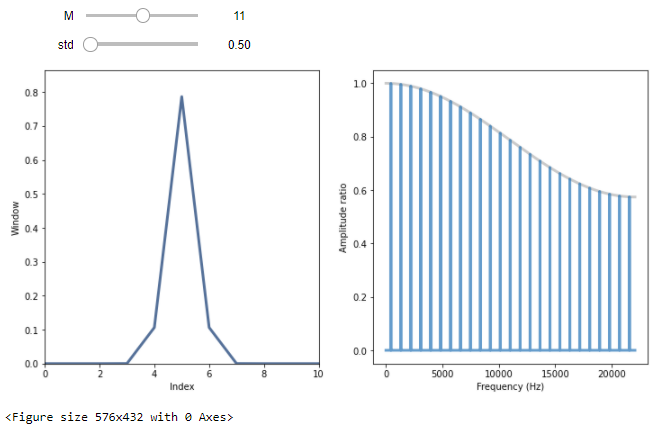
\includegraphics[width=\textwidth]{ex_1_std_0_5.png}
                \caption{\texttt{Std} = 0,5}
                \label{fig:ex_1_std_0_5}
            \end{figure}
            
            Теперь поставим \texttt{std} = 2:
            
            \begin{figure}[H]
                \centering
                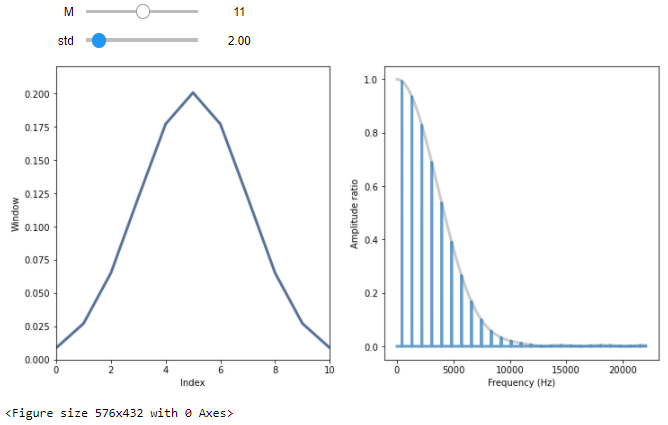
\includegraphics[width=\textwidth]{ex_1_std_2.png}
                \caption{\texttt{Std} = 2}
                \label{fig:ex_1_std_2}
            \end{figure}
            
            После этого поставим \texttt{std} = 5:
            
            \begin{figure}[H]
                \centering
                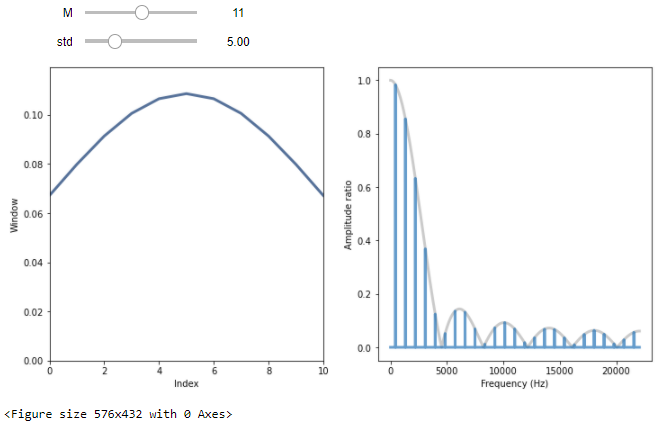
\includegraphics[width=\textwidth]{ex_1_std_5.png}
                \caption{\texttt{Std} = 5}
                \label{fig:ex_1_std_5}
            \end{figure}
            
            И, наконец, ради интереса поставим \texttt{std} = 20:
            
            \begin{figure}[H]
                \centering
                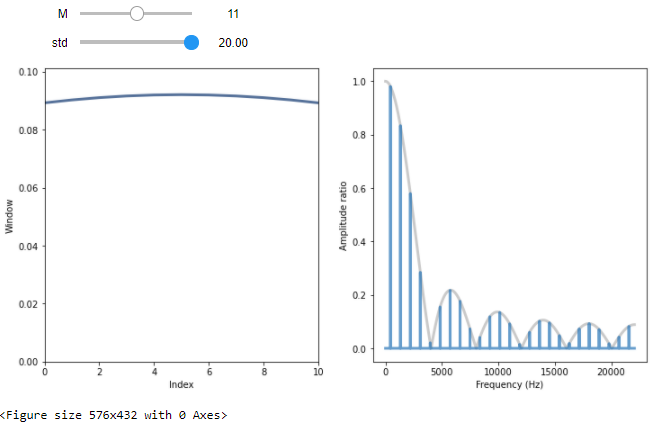
\includegraphics[width=\textwidth]{ex_1_std_20.png}
                \caption{\texttt{Std} = 20}
                \label{fig:ex_1_std_20}
            \end{figure}
            
            В итоге, на основе полученных результатов можно сделать вывод, что увеличение \texttt{std} приводит к "сплющиванию"  гауссовой кривой. 
            
    \newpage
        \section{Часть №2: Преобразование Фурье гауссовой кривой}
            Во втором пункте лабораторной работы нам необходимо попробовать ДПФ на несколких примерах и понять, что происходит при изменении \texttt{std}.
            
            Для этого создадим функцию \texttt{plot-gaussian}, которая будет отображать окно Гаусса и для него же БПФ:
            
\begin{lstlisting}[language=Python, caption= Функция \texttt{plot-gaussian}]
    def plot_gaussian(std):
        gaussian = scipy.signal.gaussian(M=32, std=std)
        gaussian /= sum(gaussian)
        
        thinkplot.preplot(num=2, cols=2)
        thinkplot.plot(gaussian)
        thinkplot.config(xlabel='Time', legend=False)
    
        fft_gaussian = np.fft.fft(gaussian)
        fft_rolled = np.roll(fft_gaussian, 32//2)
        
        thinkplot.subplot(2)
        thinkplot.plot(abs(fft_rolled))
        thinkplot.config(xlabel='Frequency')
\end{lstlisting}
            
            Также напишем интерактивный виджет для взаимодействия с данной функцией:
            
\begin{lstlisting}[language=Python, caption= Интерактивный виджет для функции \texttt{plot-gaussian}]
    slider = widgets.FloatSlider(min=0.1, max=10, value=2)
    interact(plot_gaussian, std=slider);
\end{lstlisting}
            
            Теперь с помошью данного виджета посмотрим, как будут меняться окно Гаусса и БПФ при изменении \texttt{std}:
            
            Сначала сделаем \texttt{std} = 0,5:
            
            \begin{figure}[H]
                \centering
                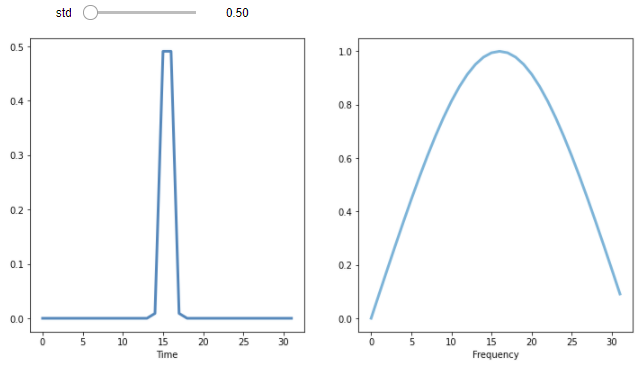
\includegraphics[width=\textwidth]{ex_2_std_0_5.png}
                \caption{\texttt{Std} = 0,5}
                \label{fig:ex_2_std_0_5}
            \end{figure}
            
            После чего сделаем \texttt{std} = 2:
            
            \begin{figure}[H]
                \centering
                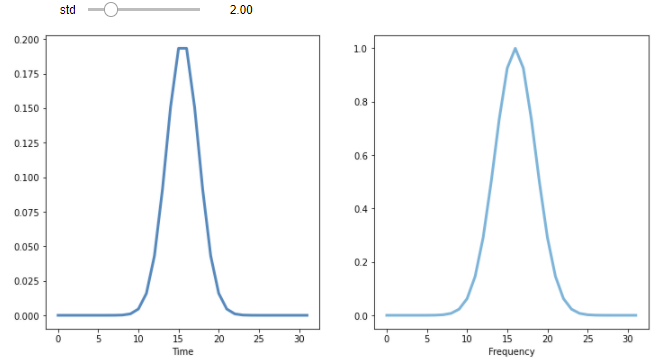
\includegraphics[width=\textwidth]{ex_2_std_2.png}
                \caption{\texttt{Std} = 2}
                \label{fig:ex_2_std_2}
            \end{figure}
            
            Затем сделаем \texttt{std} = 5:
            
            \begin{figure}[H]
                \centering
                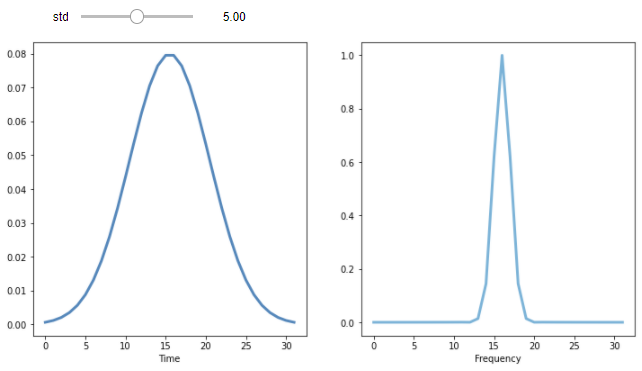
\includegraphics[width=\textwidth]{ex_2_std_5.png}
                \caption{\texttt{Std} = 5}
                \label{fig:ex_2_std_5}
            \end{figure}
            
            И, наконец, сделаем максимальное \texttt{std} = 10:
            
            \begin{figure}[H]
                \centering
                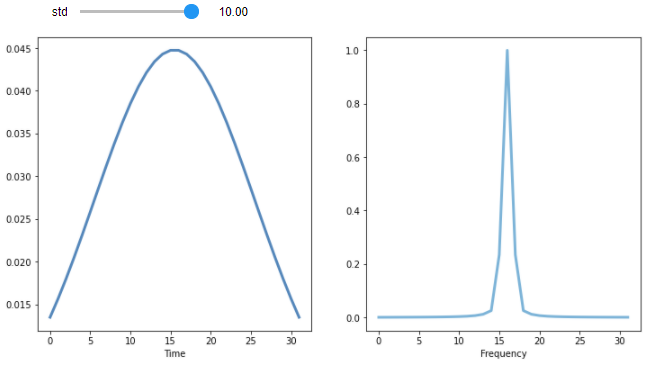
\includegraphics[width=\textwidth]{ex_2_std_10.png}
                \caption{\texttt{Std} = 10}
                \label{fig:ex_2_std_10}
            \end{figure}
            
            По итогу, при просмотре полученных результатов становится понятно, что при увеличении ширины сигнала, идет уменьшение ширины преобразования Фурье. Это работает так же и наоборот.
            
    \newpage
        \section{Часть №3: \texttt{NumPy}}
            В третьем пункте лабораторной работы нам необходимо в дополнение к Гауссову окну, использованному ранее создать окно Хэмминга тех же размеров. Также нужно дополнить окно нулями и напечатать его ДПФ. Определить, какое окно больше подходит для фильтра НЧ.
            
            Для решения данной задачи напишем функцию \texttt{plot-window}:
            
\begin{lstlisting}[language=Python, caption= Функция \texttt{plot-window}]
    def plot_window(ax, window_fun, M=30):
        signal = SquareSignal(freq=440)
        wave = signal.make_wave(duration=1.0, framerate=44100)
        
        window = window_fun(M)
        window /= sum(window)
        
        padded = zero_pad(window, len(wave))
        fft = np.fft.rfft(padded)
        
        ax[0].plot(window, label=window_fun.__name__)
        ax[1].plot(abs(fft)[:8000], label=window_fun.__name__)
        plt.legend()
        
    _, ax = plt.subplots(1, 2)
    for w in [np.blackman, np.bartlett, np.hamming, np.hanning]:
        plot_window(ax, w)
\end{lstlisting}
            
            Запустим данную функцию и посмотрим на полученный результат:
            
            \begin{figure}[H]
                \centering
                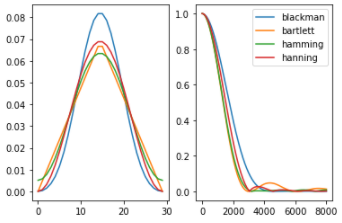
\includegraphics[width=\textwidth]{ex_3_result.png}
                \caption{Результат работы \texttt{plot-window}}
                \label{fig:ex_3_result}
            \end{figure}
            
            Как можно увидеть из результата работы функции, для фильтрации НЧ лучше всего использовать окно Хэмминга, т.к. оно дает меньше "выпуклостей".
            
            
    \newpage
        \section{Выводы}
             В результате выполнения лабораторной работы мы разобрались с тем, как ширина гауссова окна \texttt{std} влияет на гауссову кривую. Кроме того мы написали функции \texttt{plot-gaussian} и \texttt{plot-window} для отображения окна Гаусса с выводом БПФ для него и для отображения окна Хэмминга соответственно. В результате было установлено, что для фильтрации НЧ лучше всего использовать окно Хэмминга.
            
\end{document}
